
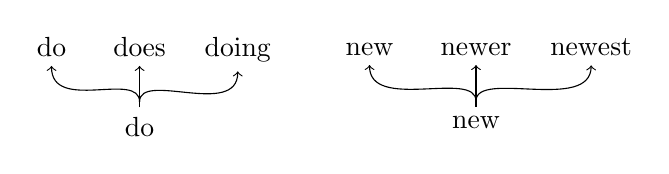
\begin{tikzpicture}
\node[] (do) at (0,0) {{\red do}}; 
\node[anchor = west] (does) at ([xshift = 1em]do.east) {{\red do}es};
\node[anchor = west] (doing) at ([xshift = 0.7em,yshift = -0.1em]does.east) {{\red do}ing};
\node[anchor = north] (do_root) at ([yshift = -1.5em]does.south) {do};

\node[anchor = west] (new) at ([xshift = 2em]doing.east) {{\red new}}; 
\node[anchor = west] (newer) at ([xshift = 1em]new.east) {{\red new}er};
\node[anchor = west] (newest) at ([xshift = 0.7em,yshift = 0.08em]newer.east) {{\red new}est};
\node[anchor = north] (new_root) at ([yshift = -1.5em]newer.south) {new};
\draw [->] ([yshift=0.2em]do_root.north) .. controls +(north:0.4) and +(south:0.6) ..(do.south);
\draw [->] (do_root.north) -- (does.south);
\draw [->] ([yshift=0.2em]do_root.north) .. controls +(north:0.4) and +(south:0.6) ..(doing.south);
\draw [->] ([yshift=0.2em]new_root.north) .. controls +(north:0.4) and +(south:0.6) ..(new.south);
\draw [->] (new_root.north) -- (newer.south);
\draw [->] ([yshift=0.2em]new_root.north) .. controls +(north:0.4) and +(south:0.6) ..(newest.south);
\end{tikzpicture}